\documentclass[landscape,a0,final]{a0poster}
\usepackage[dvipsnames,svgnames]{xcolor}
\usepackage{tikzposter} % here most of the things are defined
% change parameters only after this line You can also start a new column with an arbitrary 
% x-coordinate by specifying explicitly the coordinate of the new block node as follows:
\usepackage[czech]{babel}
\usepackage[utf8]{inputenc}
\usepackage{wrapfig}
\usepackage{url}

%Used for better control on code display

\usepackage[margin=\margin cm, paperwidth=197cm, paperheight=100cm]{geometry}

% \setbackgrounddarkcolor{ForestGreen!70!black}
% \setbackgroundlightcolor{YellowGreen!90!}

% \setfirstcolor{YellowGreen!80!}
% \setsecondcolor{gray!80!}
% \setthirdcolor{red!80!black}

\title{Improving the Apollo 12 landing site mapping\\with Chandrayaan $M^3$ data}
\author{Yann Chemin$^{1,2}$, Ian Crawford$^1$, Roberto Bugiolacchi$^1$, Huma Irfan$^1$ and Louise Alexander$^1$\\
$^1$Birkbeck College, University of London, U.K. ~ $^2$IWMI, Pelawatte, Sri Lanka}

\usetemplate{1}
\setinstituteshift{1}

\setblocktitleheight{2}
\setblockspacing{1}

\begin{document}
\ClearShipoutPicture
\AddToShipoutPicture{\BackgroundPicture}
\noindent
\tikzstyle{every picture}+=[remember picture]
\begin{tikzpicture}
\initializesizeandshifts
\titleblock{90}{1}
% \setblocktitleheight{1}

%\addlogo[north west]{(2,-1)}{9cm}{./svg_images/Grass_GIS.pdf}
%\addlogo[north east]{(-2,-2.5)}{11cm}{./svg_images/IWMI_logo.pdf}

%%%%%%%%%%%%%%%%%%%%%%%%%%%%%%%%%%%%%%%%%%%%%%%%%%%%%%%%%%%%%%%%%%%%%%%%%%%%%%%%
\blocknode{Abstract}{
\small \noindent The geology of the Apollo 12 landing site has been the subject of many studies, including recently by Korotev et al. (2011) and Snape et al. (2013). This research attempts to bring additional understanding from a remote sensing perspective using the Moon Mineralogy Mapper ($M^3$) sensor data, onboard the Chandrayaan lunar orbiter. This has a higher spatial-spectral resolution sensor than the Clementine UV-Vis sensor and provides the opportunity to study the lunar surface with detailed spectral signatures.\newline

Mapping of FeO (wt\%) and TiO 2 (wt\%) is done using the methods of Lucey et al. (2000) and Wilcox et
al. (2005). A FeO \& TiO 2 processing module (i.feotio2) is made specifically for this research within the Free \& Open Source Software GRASS GIS (Neteler et al., 2012). Attempts will be made to estimate the lava flow thickness using the method of Bugiolacchi et al. (2006) and individual lava layers thicknesses (Weider et al., 2010). Integration of this new information will be put in perspective and integrated with previous work. Analysis from the combined higher spatial and spectral resolutions will improve the accuracy of the geological mapping at the Apollo 12 landing site.\newline
}


%%%%%%%%%%%%%%%%%%%%%%%%%%%%%%%%%%%%%%%%%%%%%%%%%%%%%%%%%%%%%%%%%%%%%%%%%%%%%%%%
\blocknode{Previous interpretations}{
Korotev et al. (2011) reviewed the lunar research done until recently, with a special interest in the Apollo 12 landing site and its vicinity. Among the information newly deducted, are a geological context block diagram 1 (Figure below) along with an Apollo 12 landing site interpretive cross-section. Fortezzo and Hare (2013) completed the digital renovation of the 1:5,000,000 lunar geological maps series, enhanced with LOLA-LRO information.\newline
\begin{center}
	\begin{tabular}{cc}
		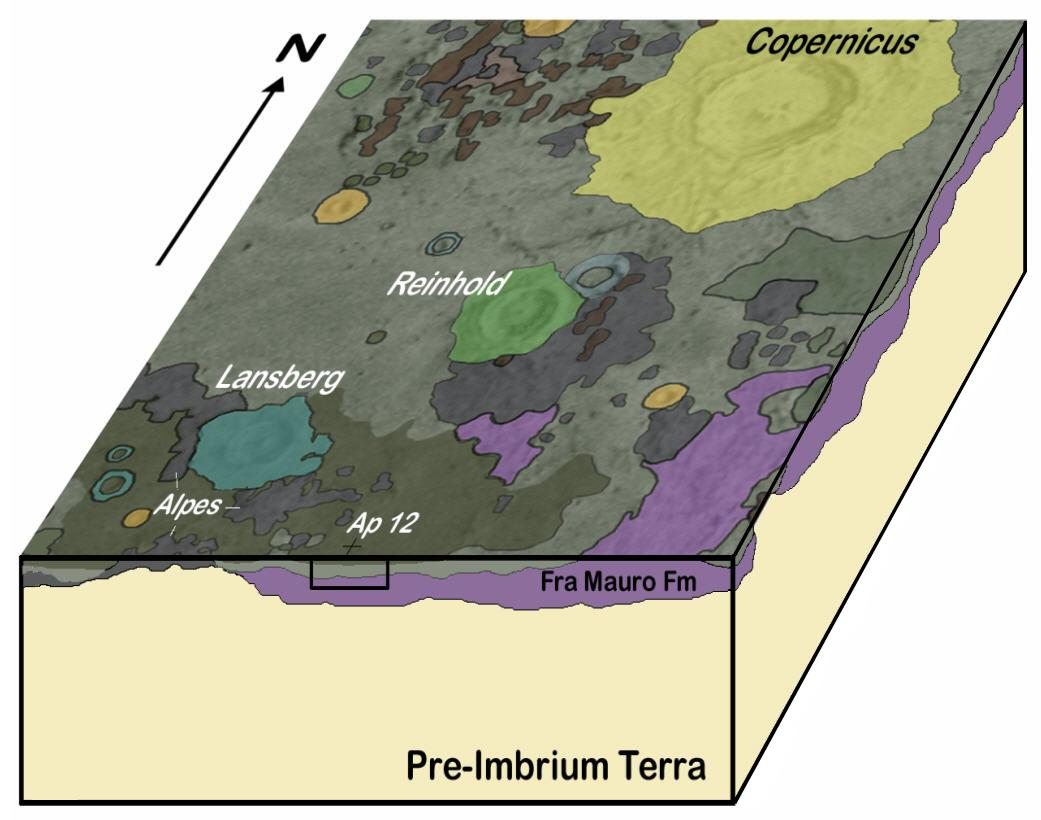
\includegraphics[width=0.45\textwidth]{./images/Korotev_block}
		&
		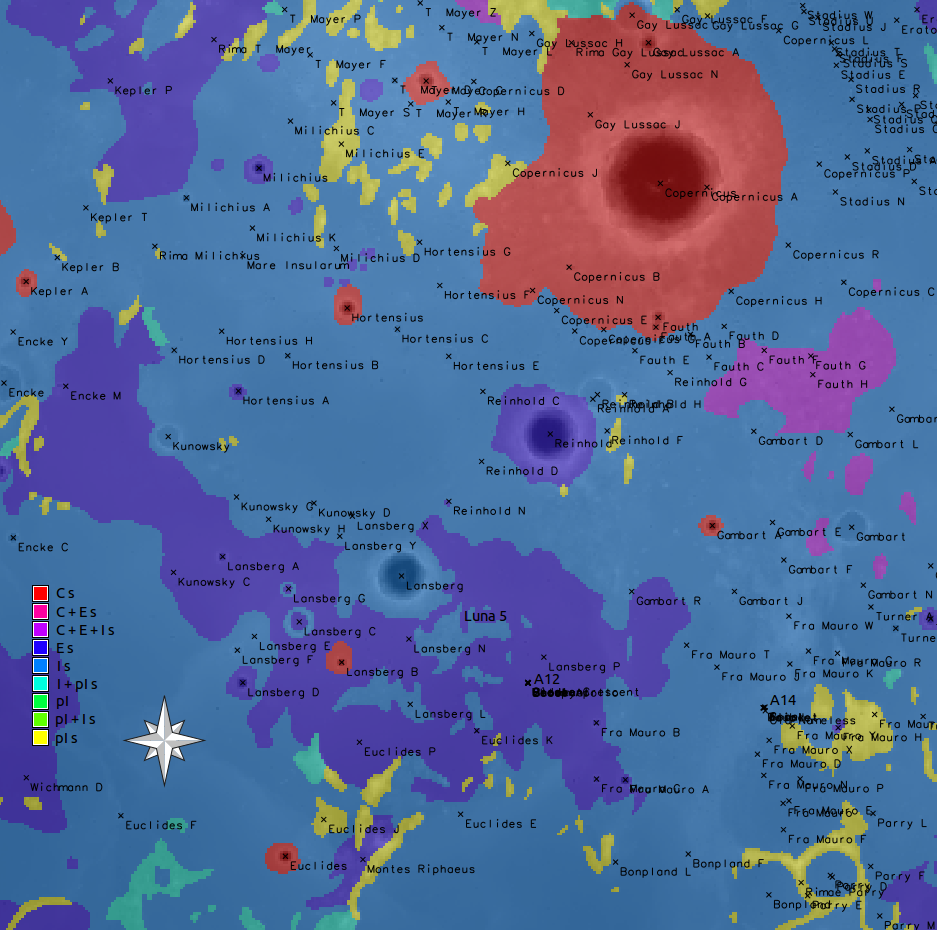
\includegraphics[width=0.45\textwidth]{./images/A12region}
	\end{tabular}\newline
Figure 2: a) Korotev et al (2011) geological block of Apollo 12 landing site\\
b)  Fortezzo and Hare (2013) geological maps series with moon nomenclature.
\end{center}
}


%%%%%%%%%%%%%%%%%%%%%%%%%%%%%%%%%%%%%%%%%%%%%%%%%%%%%%%%%%%%%%%%%%%%%%%%%%%%%%%%
\getcurrentrow{box}
\coordinate (funkcionalita) at (box.south west);
\coordinate (funkcionalitaeast) at (box.east);
\coordinate (screenshot) at (box.north west);

\blocknodew[($(funkcionalita)+(20,-1)$)]{35}{References}{
\scriptsize
\begin{flushleft}
\begin{tabular}{rp{0.9\textwidth}}
Bugiolacchi et al. (2006) &  Planetary Science. 41(2):285-304.\\{}
Fortezzo et al. (2013) & LPI Contributions, 1719:2114.\\{}
Korotev et al. (2011) & Geochimica et Cosmochimica Acta. 75(6):1540-1573.\\{}
Lucey et al. (2000) & J. Geophys. Res. 105(E8): 20297-20305.\\{}
Neteler et al. (2012) & Environment \& Modeling Software, 31:124-130.\\{}
Snape et al. (2013) & LPSC Abstracts 44:1044.\\{}
Weider et al. (2010) & Icarus, 209, 323-336.\\{}
Wilcox et al. (2005) & J. Geophys. Res. 110(E11):2156-2202.\\{}
Zhang et al. (2013) & LPSC Abstracts 44:374.\\{}
\end{tabular}
\end{flushleft}
\smallskip
\hrulefill
\vspace{-5pt}

\begin{center}
\begin{tabular}{cp{0.9\textwidth}}
\begin{minipage}{0.15\textwidth}

\includegraphics[width=0.7in]{./images/grass_qr.pdf}
\end{minipage}

\begin{minipage}{0.3\textwidth}
\small {\url{www.bbk.ac.uk}}
\end{minipage}

\begin{minipage}{0.15\textwidth}

\includegraphics[width=0.7in]{./images/grass_qr.pdf}
\end{minipage}

\begin{minipage}{0.3\textwidth}
\small {\url{grass.osgeo.org}}
\end{minipage}
\end{tabular}
\end{center}

\hrulefill
\vspace{14pt}
\begin{center}
\newcommand{\logowidth}{5em}
\newcommand{\logospace}{\hspace{0.1em}}
\noindent

\includegraphics[width=\logowidth]{./svg_images/public_domain_logo.pdf}
%\raisebox{0.7\height}{\logospace 2013 GRASS Development Team}
\end{center}
}

\startsecondcolumn
%%%%%%%%%%%%%%%%%%%%%%%%%%%%%%%%%%%%%%%%%%%%%%%%%%%%%%%%%%%%%%%%%%%%%%%%%%%%%%%%
\blocknode{Clementine data}{
\smallskip

\begin{center}
 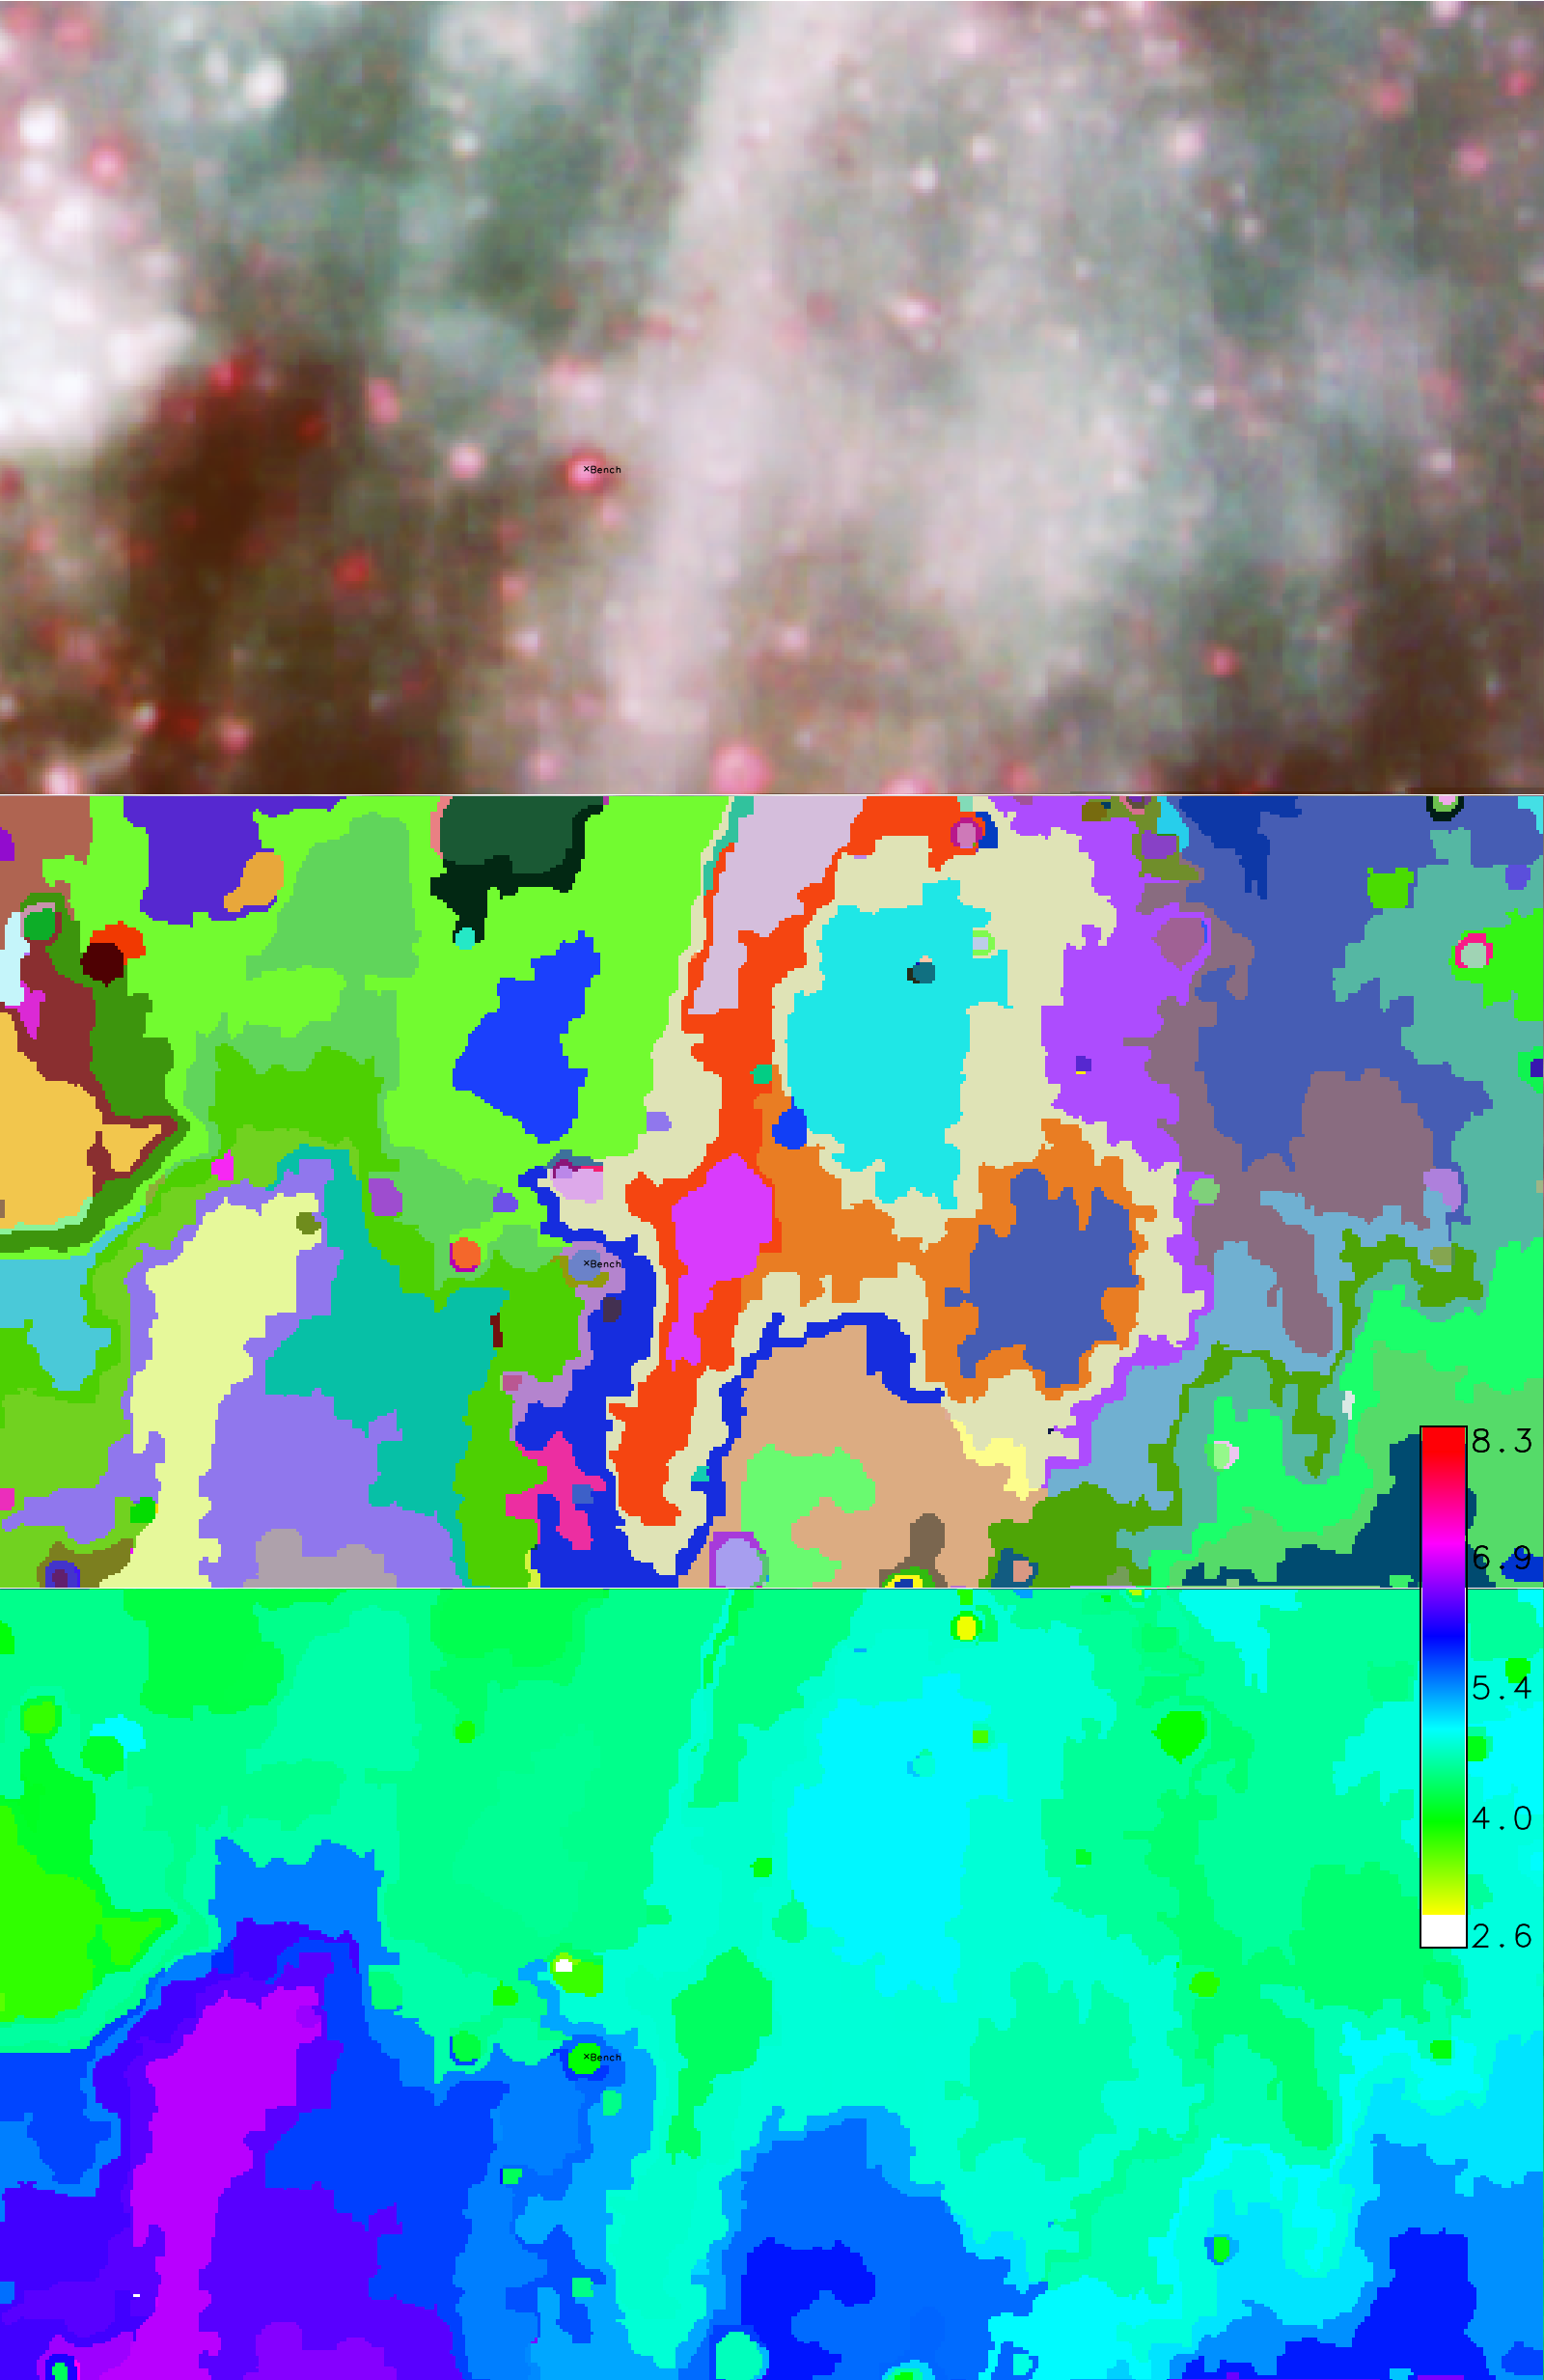
\includegraphics[width=0.75\textwidth]{./images/Clementine}
 \newline
 Figure 1: Clementine RGB153 (top), segmentation (middle) and FeO (wt\%) per segmentation class (bottom).
\end{center}
}



\startthirdcolumn
%%%%%%%%%%%%%%%%%%%%%%%%%%%%%%%%%%%%%%%%%%%%%%%%%%%%%%%%%%%%%%%%%%%%%%%%%%%%%%%
\blocknode{M$^3$ Signal at Apollo 12 landing site}{
\smallskip
\begin{center}
\begin{tabular}{ c p{0.45\textwidth}}
 \raisebox{-1.2\totalheight}{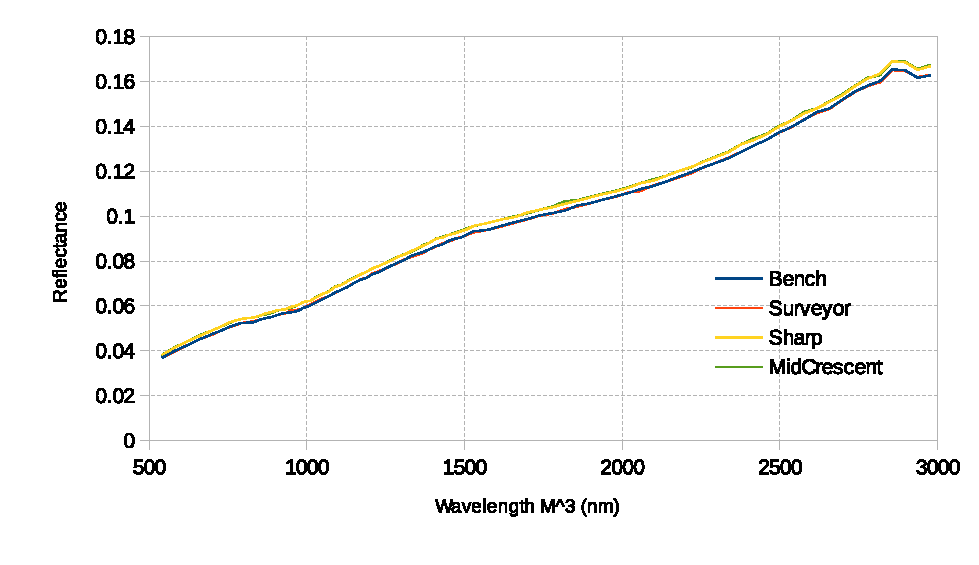
\includegraphics[width=0.5\textwidth]{./images/M3_A12_craters_signal}}\newline
 %\caption{Spectral signature of $M^3$ from four craters}
 \label{fig:specsignature4craters}
 &
 \noindent Chandrayaan $M^3$ data was  downloaded from PDS \url{http://pds-imaging.jpl.nasa.gov/}{pds-imaging.jpl.nasa.gov}. The tile \textit{M3G20090111T013904\_V01\_RFL.IMG} was imported in GRASS GIS, resulting in 85 bands. The spectrum for four craters where extracted in the Figure \ref{fig:specsignature4craters}. Bench and Surveyor are both together in the lower reflectance curves. On the higher side, Sharp and Middle Crescent are consistently above the two others. This higher broadband Albedo is increasing towards the West, where one of the ray is clearly drawn (Oblique white strip in the middle of The Clementine upper map. Compared to the spectral data from Figure ~\ref{fig:specsignatureASTERlib} the reflectance is overall lower and the obvious shape differences are there.
 \end{tabular}
 \end{center}
 \begin{flushleft}
 \hspace{22mm}
 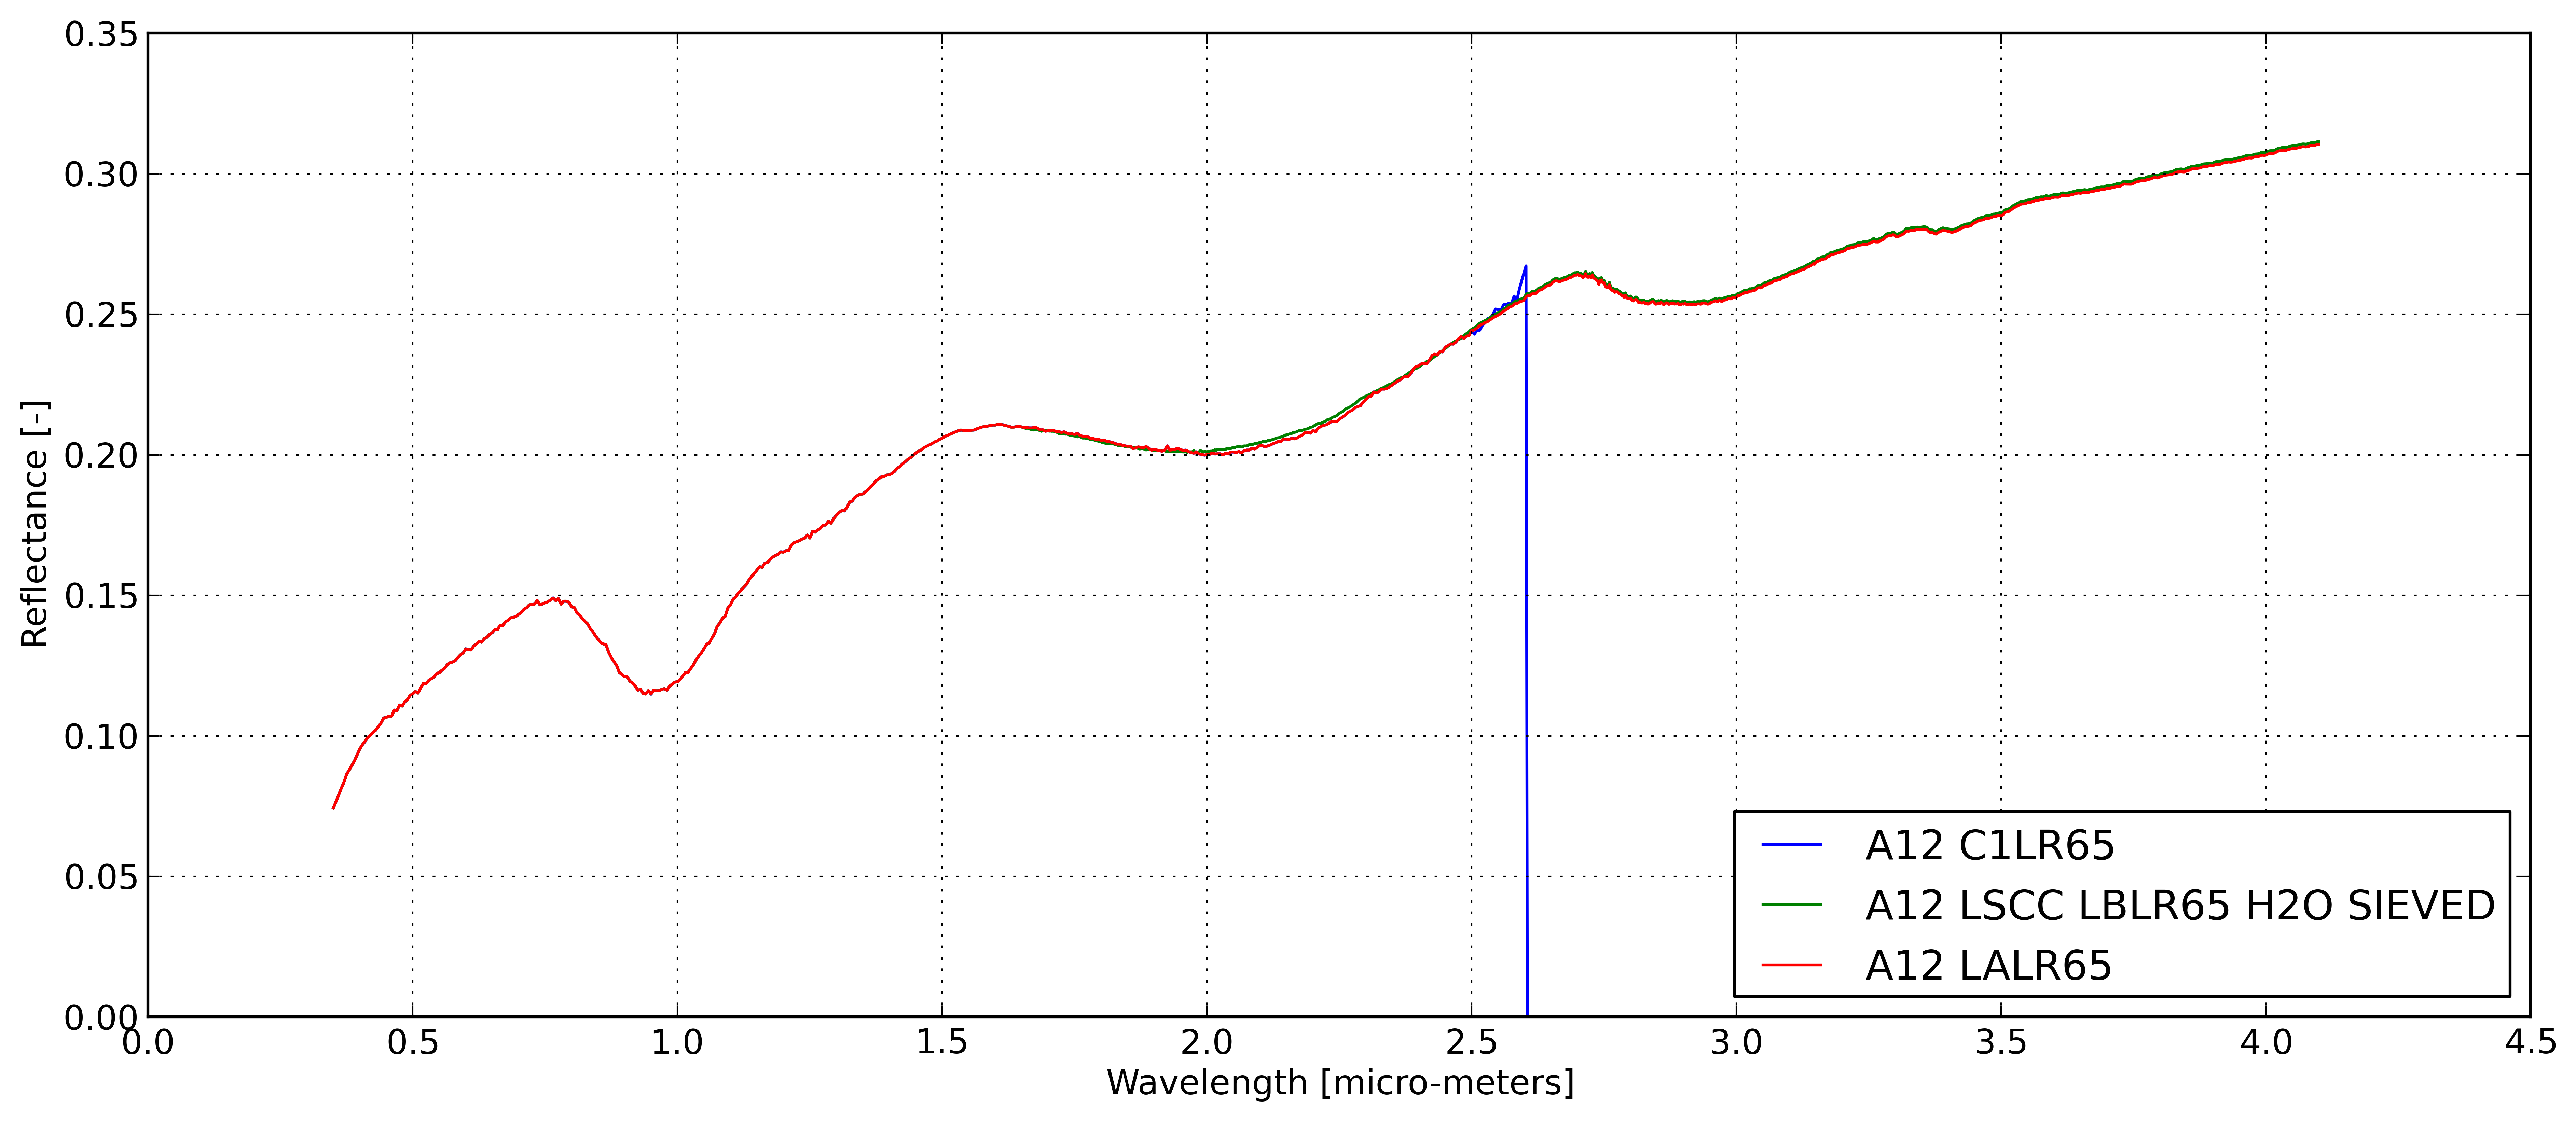
\includegraphics[width=0.45\textwidth]{./images/Apollo12_signatures}
 %\caption{Spectral signature from Apollo 12 (ASTER library)}
 \label{fig:specsignatureASTERlib}
 \end{flushleft}

}


\startfourthcolumn
%%%%%%%%%%%%%%%%%%%%%%%%%%%%%%%%%%%%%%%%%%%%%%%%%%%%%%%%%%%%%%%%%%%%%%%%%%%%%%%%
\blocknode{M$^3$ derived FeO from standard equations}{
\noindent The wt\%FeO equations have a large range of results when used with $M^3$ data:
\begin{center}
\begin{tabular}{ l r r}
\hline
Authors & Bench & Surveyor\\
\hline
Lucey et al. (2000) & -26.64 & -23.32 \\
Lawrence et al. (2002) & 4.72 & 6.38 \\
Wilcox et al. (2005) & 22.28 & 21.82 \\
Zhang et al. (2013) & 19.74 & 19.49 \\
\hline
\end{tabular}
\end{center}
\bigskip

\begin{center}
\begin{tabular}{ c p{0.45\textwidth}}
 \raisebox{-0.8\totalheight}{\includegraphics[width=0.5\textwidth]{./code/code1}}
 %\caption{Testing FeO algorithms.}
 \label{fig:FeOtesting}
 &
 \noindent It is known that the local range of FeO is below 10wt\% from UVVIS data (see Figure on the lower left), only the Lawrence et al. (2002) equation is giving an appropriate range. Lucey et al. (2000) equation fails because of the offset of uvvis4/uvvis2(=1.15 vs offset = 1.19) and the one for uvvis2(=0.05 vs offset = 0.08), as both of the parts are negative thus giving a positive division output, their interplay should bring a negative number for the arctangent negative sign to compensate. This clearly does not happen with $M^3$ data in the Bench and Surveyor craters, the results from the arctangent being positive, and the sign change brings the main part of the equation to a negative, further reduced by the negative final offset.\newline
\end{tabular}
\end{center}
\noindent Upon using the  Lawrence et al. (2002) equation, it turned out that though the wt\%FeO range was satisfactory for few crater points, the rate of change was actually reverse to the expected one, reducing to null towards the South of the landing site and increasing towards the North.\newline
\noindent The equation from Zhang et al. (2013) is giving an appropriate rate of change, however, the local values are too large compared to the Clementine derived FeO values.\newline

}



\end{tikzpicture}

\end{document}
